% =====================================================================
%  Section IV — Dataset Construction
%  Replaces Section IV of Research_Paper_version01_6 in full.
%
%  CITATION KEYS: these match the named \bibitem labels in main_v6.tex
%  (midv, idnet, sidtd, doctamper, cmid, tesseract, uidai-scheme).  ONE key,
%  `augraphy`, has no \bibitem in main_v6.tex yet -- add this to
%  thebibliography, or delete the single sentence that cites it in
%  Section IV-F:
%
%    \bibitem{augraphy} A. Groleau, K. W. Chee, S. Larson, S. Maini, and
%    J. Boarman, ``Augraphy: A Data Augmentation Library for Document
%    Images,'' in \emph{Proc. Int. Conf. Document Analysis and Recognition
%    (ICDAR)}, Lecture Notes in Computer Science, vol. 14191, Springer,
%    2023, pp. 384--401.
%
%  Requires, in the preamble:
%     \usepackage{booktabs}
%     % Auto-generated by scripts/export_latex.py -- do not edit by hand.
\newcommand{\dsPersons}{300}
\newcommand{\dsDocuments}{3600}
\newcommand{\dsImages}{10800}
\newcommand{\dsGenuine}{3600}
\newcommand{\dsForged}{7200}
\newcommand{\dsGiB}{0.87}
\newcommand{\dsNq}{3}
\newcommand{\dsTrainImg}{7560}
\newcommand{\dsValImg}{1620}
\newcommand{\dsTestImg}{1620}
\newcommand{\dsTrainPer}{210}
\newcommand{\dsValPer}{45}
\newcommand{\dsTestPer}{45}
\newcommand{\dsCellImages}{900}
\newcommand{\dsCellControls}{1800}
\newcommand{\dsPhashBits}{256}
\newcommand{\dsPhashDistinctSixtyFour}{5824}
\newcommand{\dsPhashDistinct}{10757}
\newcommand{\dsPhashAUC}{0.951}
\newcommand{\dsPhashOverlap}{2.3}
\newcommand{\dsPhashWithinMed}{30}
\newcommand{\dsPhashCrossPersonMed}{108}
\newcommand{\dsPhashCrossPersonMin}{6}
\newcommand{\dsAadhaarSpace}{8\times10^{10}}
\newcommand{\dsPanSpace}{4.6\times10^{10}}
\newcommand{\dsAadhaarStrings}{1083}
\newcommand{\dsPanStrings}{1200}
\newcommand{\dsAadhaarCoinPct}{1.8}
\newcommand{\dsAadhaarCoinExp}{19}
\newcommand{\dsPanCoinPct}{1.8}
\newcommand{\dsPanCoinExp}{21}
\newcommand{\dsStrictAll}{9.0}
\newcommand{\dsStrictInitialFirst}{29.3}
\newcommand{\dsStrictLeadingInitial}{93.1}
\newcommand{\dsCICell}{2.0}
\newcommand{\dsCIPerson}{3.4}
\newcommand{\dsFPAadhaarClean}{0.3}
\newcommand{\dsFPAadhaarMild}{0.3}
\newcommand{\dsFPAadhaarSevere}{11.7}
\newcommand{\dsFPAadhaarAll}{4.1}
\newcommand{\dsFPPanClean}{12.7}
\newcommand{\dsFPPanMild}{12.2}
\newcommand{\dsFPPanSevere}{31.8}
\newcommand{\dsFPPanAll}{18.9}
\newcommand{\dsOcrAadhaarAadhaarNumberClean}{99.8}
\newcommand{\dsOcrAadhaarAadhaarNumberMild}{99.4}
\newcommand{\dsOcrAadhaarAadhaarNumberSevere}{88.3}
\newcommand{\dsOcrPanPanNumberClean}{85.2}
\newcommand{\dsOcrPanPanNumberMild}{84.9}
\newcommand{\dsOcrPanPanNumberSevere}{67.7}
\newcommand{\dsOcrAadhaarNameClean}{98.8}
\newcommand{\dsOcrAadhaarNameMild}{98.7}
\newcommand{\dsOcrAadhaarNameSevere}{64.7}
\newcommand{\dsOcrPanNameClean}{99.7}
\newcommand{\dsOcrPanNameMild}{99.6}
\newcommand{\dsOcrPanNameSevere}{53.8}
\newcommand{\dsProbeRecords}{40}
\newcommand{\dsProbeCells}{8}
\newcommand{\dsProbeComparisons}{320}
\newcommand{\dsProbeOutside}{0}
\newcommand{\dsProbeCritical}{0.500}
\newcommand{\dsProbeCriticalAUC}{0.493}
\newcommand{\dsProbeCriticalN}{1080}
\newcommand{\dsProbeCriticalCI}{$[0.470,\,0.530]$}
\newcommand{\dsProbeControl}{0.491}
\newcommand{\dsProbeControlAUC}{0.494}
\newcommand{\dsProbeControlN}{540}
\newcommand{\dsProbeControlCI}{$[0.449,\,0.533]$}
\newcommand{\dsProbeCriticalClean}{0.492}
\newcommand{\dsProbeCriticalCleanAUC}{0.491}
\newcommand{\dsProbeCriticalCleanN}{360}
\newcommand{\dsProbeCriticalCleanCI}{$[0.440,\,0.543]$}
\newcommand{\dsProbeControlClean}{0.506}
\newcommand{\dsProbeControlCleanAUC}{0.454}
\newcommand{\dsProbeControlCleanN}{180}
\newcommand{\dsProbeControlCleanCI}{$[0.433,\,0.579]$}
          % auto-generated macros
%  and, where the tables are placed:
%     \begin{table*}[t]
\caption{Forgery categories, their intended
detectability, and the realised image counts per document type.
$\dsCellControls$ control images per document type comprise two
unmodified renders of every record at $\dsNq$ quality tiers. C2, C3
and C4 are produced by re-rendering from a modified record, so they
carry no pixel-level trace; C1 is the only category in which pixels
are edited after rendering, and it leaves every printed value valid.}
\label{tab:forgery}
\centering
\footnotesize
\begin{tabular}{@{}l p{7.2cm} l p{2.7cm} r r@{}}
\toprule
Cat. & Construction & Visual branch & Rule branch & Aadhaar & PAN \\
\midrule
C0 & Unmodified render & pass & pass & 1800 & 1800 \\
C1 & Post-render pixel edit; every printed value remains valid & detect & pass & 900 & 900 \\
C2 & Re-render with a structurally invalid identifier: Aadhaar checksum broken, or PAN format or category character broken & miss & detect & 900 & 900 \\
C3 & Re-render with a semantically inconsistent field pair: PAN fifth character against the name, Aadhaar Latin against Devanagari name & miss & detect (PAN only) & 900 & 900 \\
C4 & Re-render with a fabricated identifier that satisfies every rule & miss & miss & 900 & 900 \\
\bottomrule
\end{tabular}
\end{table*}

%     \begin{table}[t]
\caption{Per-field OCR extraction quality by capture quality tier:
exact-match rate with a 95\% Wilson interval, and mean character
error rate. Raw Tesseract output, with only the parsing step of
Section~\ref{subsec:ocr} applied.}
\label{tab:ocr}
\centering
\footnotesize
\begin{tabular}{@{}llrrr@{}}
\toprule
Field & Tier & $n$ & Exact match \% [95\% CI] & CER \% \\
\midrule
A: number & clean & 1800 & 99.8 [99.5, 99.9] & 0.01 \\
 & mild & 1800 & 99.4 [99.0, 99.7] & 0.07 \\
 & severe & 1800 & 88.3 [86.8, 89.7] & 2.50 \\
\addlinespace[1.5pt]
A: name & clean & 1800 & 98.8 [98.2, 99.2] & 0.10 \\
 & mild & 1800 & 98.7 [98.1, 99.2] & 0.10 \\
 & severe & 1800 & 64.7 [62.5, 66.9] & 22.22 \\
\addlinespace[1.5pt]
A: DOB & clean & 1800 & 100.0 [99.8, 100.0] & 0.00 \\
 & mild & 1800 & 100.0 [99.8, 100.0] & 0.00 \\
 & severe & 1800 & 41.5 [39.2, 43.8] & 45.33 \\
\addlinespace[1.5pt]
P: number & clean & 1800 & 85.2 [83.5, 86.7] & 1.57 \\
 & mild & 1800 & 84.9 [83.2, 86.5] & 1.57 \\
 & severe & 1800 & 67.7 [65.5, 69.8] & 7.30 \\
\addlinespace[1.5pt]
P: name & clean & 1800 & 99.7 [99.3, 99.8] & 0.04 \\
 & mild & 1800 & 99.6 [99.2, 99.8] & 0.06 \\
 & severe & 1800 & 53.8 [51.5, 56.1] & 31.78 \\
\addlinespace[1.5pt]
P: father & clean & 1800 & 100.0 [99.8, 100.0] & 0.00 \\
 & mild & 1800 & 100.0 [99.8, 100.0] & 0.00 \\
 & severe & 1800 & 44.7 [42.4, 47.0] & 43.68 \\
\addlinespace[1.5pt]
P: DOB & clean & 1800 & 99.7 [99.3, 99.9] & 0.03 \\
 & mild & 1800 & 99.9 [99.7, 100.0] & 0.01 \\
 & severe & 1800 & 33.8 [31.7, 36.0] & 50.84 \\
\bottomrule
\end{tabular}
\end{table}

%     \begin{table}[t]
\caption{Rule-branch flag rate by forgery category (\% of images on
which an applicable rule evaluated \textsc{false}), on ground-truth
text and on OCR-extracted text, with 95\% Wilson intervals. On C0 a
flag is a false positive. On C4 both branches are expected to miss by
construction, so a flag there is an OCR-induced false alarm and not
detection of the fabrication.}
\label{tab:rulerate}
\centering
\footnotesize
\begin{tabular}{@{}llll@{}}
\toprule
Document & Cat. & Ground-truth text & OCR text \\
\midrule
Aadhaar & C0 & 0.0 [0.0, 0.2] & 4.1 [3.3, 5.1] \\
 & C1 & 0.0 [0.0, 0.4] & 4.1 [3.0, 5.6] \\
 & C2 & 100.0 [99.6, 100.0] & 99.8 [99.2, 99.9] \\
 & C3 & 0.0 [0.0, 0.4] & 3.9 [2.8, 5.4] \\
 & C4 & 0.0 [0.0, 0.4] & 4.0 [2.9, 5.5] \\
\midrule
PAN & C0 & 0.0 [0.0, 0.2] & 18.9 [17.1, 20.8] \\
 & C1 & 0.0 [0.0, 0.4] & 20.8 [18.3, 23.5] \\
 & C2 & 100.0 [99.6, 100.0] & 97.1 [95.8, 98.0] \\
 & C3 & 100.0 [99.6, 100.0] & 96.2 [94.8, 97.3] \\
 & C4 & 0.0 [0.0, 0.4] & 23.2 [20.6, 26.1] \\
\bottomrule
\end{tabular}
\end{table}

%     \begin{table}[t]
\caption{Rule-branch false-positive rate on \emph{genuine} documents
(category C0) as a function of capture quality, evaluated on
OCR-extracted text. On ground-truth text the rate is zero by
construction, so every entry here is attributable to OCR extraction
error. This is the measurement RQ6 requires.}
\label{tab:fpr}
\centering
\footnotesize
\begin{tabular}{@{}llrrl@{}}
\toprule
Document & Tier & $n$ & FP & FP rate \% [95\% CI] \\
\midrule
Aadhaar & clean & 600 & 2 & 0.3 [0.1, 1.2] \\
 & mild & 600 & 2 & 0.3 [0.1, 1.2] \\
 & severe & 600 & 70 & 11.7 [9.3, 14.5] \\
 & all & 1800 & 74 & 4.1 [3.3, 5.1] \\
\midrule
PAN & clean & 600 & 76 & 12.7 [10.2, 15.6] \\
 & mild & 600 & 73 & 12.2 [9.8, 15.0] \\
 & severe & 600 & 191 & 31.8 [28.2, 35.7] \\
 & all & 1800 & 340 & 18.9 [17.1, 20.8] \\
\bottomrule
\end{tabular}
\end{table}

%     \begin{table}[t]
\caption{PAN cross-field rule on \emph{genuine} documents:
permissive rule (2) against the strict variant, by naming stratum and
by the source of the fifth character. A failure here is a false
positive on a genuine document. The strict variant is reported as a
sensitivity analysis, not as the study's rule.}
\label{tab:permstrict}
\centering
\scriptsize
\setlength{\tabcolsep}{3.5pt}
\begin{tabular}{@{}llrll@{}}
\toprule
Subset & Text & $n$ & Permissive FAIL \% & Strict FAIL \% \\
\midrule
all genuine PAN & gt & 1800 & 0.0 [0.0, 0.2] & 9.0 [7.8, 10.4] \\
 & ocr & 1800 & 1.9 [1.4, 2.6] & 9.4 [8.2, 10.9] \\
\addlinespace[1.5pt]
surname-last & gt & 648 & 0.0 [0.0, 0.6] & 0.0 [0.0, 0.6] \\
 & ocr & 648 & 1.1 [0.5, 2.2] & 1.4 [0.7, 2.6] \\
\addlinespace[1.5pt]
initial-first & gt & 552 & 0.0 [0.0, 0.7] & 29.3 [25.7, 33.3] \\
 & ocr & 552 & 3.8 [2.5, 5.7] & 27.4 [23.8, 31.2] \\
\addlinespace[1.5pt]
mononymic & gt & 600 & 0.0 [0.0, 0.6] & 0.0 [0.0, 0.6] \\
 & ocr & 600 & 1.0 [0.5, 2.2] & 1.7 [0.9, 3.0] \\
\addlinespace[1.5pt]
$p_5$ from initial & gt & 174 & 0.0 [0.0, 2.2] & 93.1 [88.3, 96.0] \\
 & ocr & 174 & 6.9 [4.0, 11.7] & 81.0 [74.6, 86.2] \\
\addlinespace[1.5pt]
$p_5$ from given name & gt & 378 & 0.0 [0.0, 1.0] & 0.0 [0.0, 1.0] \\
 & ocr & 378 & 2.4 [1.3, 4.5] & 2.6 [1.4, 4.8] \\
\addlinespace[1.5pt]
\bottomrule
\end{tabular}
\end{table}

%     \begin{table}[t]
\caption{Leakage audit performed on the released splits. Each check is
run on the corpus and its outcome reported, rather than asserted. The
first four checks are exact and all pass. The fifth, near-duplicate
detection by perceptual hashing, is reported as a \emph{diagnostic}
rather than a gate: on a corpus in which every document shares one
of six layout templates, the same-document and different-person
distance distributions overlap, so no threshold can separate a
leaked duplicate from two unrelated documents. See
Section~\ref{subsec:leakage} and Fig.~\ref{fig:phash}.}
\label{tab:leakage}
\centering
\scriptsize
\setlength{\tabcolsep}{3.5pt}
\begin{tabular}{@{}p{1.15cm}p{3.0cm}ll@{}}
\toprule
Leakage mode & Check & Required & Observed \\
\midrule
Identity & person-id intersection across splits & empty & 0 \\
Identifier & Aadhaar/PAN string intersection & empty & 0 \\
Template & every layout variant in every split & all & 6/6 \\
Near-duplicate & \dsPhashBits-bit perceptual-hash distance & (diagnostic) & see Sec.~\ref{subsec:leakage} \\
Augment\-ation & degradation draws of one document & one split & 0 span splits \\
Printed values & identical field-value set in two splits & none & 0 of 2100 \\
\bottomrule
\end{tabular}
\end{table}

%
%  Every numeral below comes from generated/numbers.tex, which is written by
%  scripts/export_latex.py directly from the built corpus.  Rebuild the dataset,
%  re-run the exporter, recompile: no number in this section can drift from the
%  data it describes.
% =====================================================================

\section{Dataset Construction}
\label{sec:dataset}

No public corpus pairs Aadhaar- or PAN-format document images with field-level
structural ground truth, so the incremental value this study measures cannot be
measured on existing data. MIDV-2020~\cite{midv}, IDNet~\cite{idnet} and
SIDTD~\cite{sidtd} establish that synthetic generation is the accepted substitute
for sensitive identity-document data, and this section follows that rationale
while adding what those corpora do not carry: for every image, the printed value
of every field, whether that value satisfies the rules of
Section~\ref{sec:framework}, and which field was corrupted to make it fail.

\subsection{Design Principles}
\label{subsec:principles}

Four constraints govern the construction. Each is enforced by the generation
procedure rather than checked after the fact.

\emph{First, no real document is used at any stage.} All identifiers, names,
dates of birth, photographs and signatures are synthetic, following the privacy
rationale of SIDTD~\cite{sidtd} and MIDV-2020~\cite{midv}. No generated
identifier was submitted to, resolved through, or checked against any UIDAI or
Income Tax Department service, and no real identity-document image was
collected, downloaded or processed. Section~\ref{subsec:ethics} states what this
does and does not guarantee.

\emph{Second, the layouts are format-faithful and deliberately
design-unfaithful.} They reproduce the field structure of the two documents --
which fields are printed, in what order, with what identifier grouping -- because
that structure is what the validators of Section~\ref{sec:framework} operate on.
They do not reproduce any official emblem, seal, hologram, colour scheme or
authority name; a geometric placeholder mark and a fictitious authority name
stand in their place. Three layout variants exist per document type, differing
in typeface pairing, accent colour, label placement, photograph side and
background pattern density. Every rendered image carries an identical
low-opacity \textsc{synthetic specimen} overlay, composited before any forgery
operation and drawn identically for all categories, so that it cannot act as a
class-correlated cue. This choice costs realism and buys two things: the
released artefacts cannot function as documents, and the study is not obliged to
defend a pixel-level reproduction of a government design.

\emph{Third, the templates are authored rather than obtained.} Because no public
corpus supplies Aadhaar or PAN images with field-level structural ground truth,
both layouts were written as parameterised vector layouts and rasterised
directly. Exact field bounding boxes are therefore a by-product of rendering
rather than an annotation task, and they are propagated through the degradation
homography of Section~\ref{subsec:degrade} so that a field can be read from the
\emph{same pixels} both as ground truth and through OCR. That correspondence is
what makes the RQ4 comparison possible at all.

Figure~\ref{fig:pipeline} shows how the stages fit together and
Algorithm~\ref{alg:dataset} states the procedure as implemented.

\emph{Fourth, and most consequentially for the experimental claim, the forgery
categories intended to be visually undetectable are produced by re-rendering the
document from a modified identity record, not by editing a rendered image}, and
from the \emph{same render seed} as the genuine control, so that before
degradation the two images are identical outside the corrupted field. This is
developed in Section~\ref{subsec:taxonomy} and verified exactly in
Section~\ref{subsec:probe}.


\begin{figure*}[!t]
\centering
\resizebox{\textwidth}{!}{%
\begin{tikzpicture}[
  font=\scriptsize,
  box/.style={draw, rounded corners=2pt, align=center, minimum height=9mm,
              inner xsep=3pt, text width=20mm, fill=black!4},
  gen/.style={box, fill=blue!7},
  frg/.style={box, fill=red!7},
  aud/.style={box, fill=green!9},
  ar/.style={-{Latex[length=1.6mm]}, thick}
]
\node[gen] (rec)  at (0,0)    {Identity records\\{\tiny §\,IV-C: identifiers,\\names, strata}};
\node[gen] (spl)  at (2.55,0) {Grouped split\\{\tiny §\,IV-J: by person}};
\node[gen] (base) at (5.1,0)  {Base render\\{\tiny §\,IV-A: seed $b$,\\field boxes}};
\node[frg] (forg) at (7.75,0) {Forgery injection\\{\tiny §\,IV-E: C0--C4}};
\node[box] (deg)  at (10.5,0) {Degradation\\{\tiny §\,IV-G: 3 tiers,\\seed independent}};
\node[box] (ocr)  at (13.2,0) {Per-field OCR\\{\tiny §\,IV-H: crop to\\mapped boxes}};
\node[box] (val)  at (15.9,0) {Validators\\{\tiny §\,III on GT text\\and on OCR text}};
\node[aud] (pre)  at (7.75,1.55) {Pre-flight assertion\\{\tiny §\,IV-E: expected\\rule outcome holds}};
\node[aud] (prb)  at (5.1,-1.55) {Renderer-leakage\\probe {\tiny §\,IV-F}};
\node[aud] (lk)   at (10.5,-1.55) {Leakage audits\\{\tiny §\,IV-J, Table~\ref{tab:leakage}}};
\node[box] (man)  at (15.9,-1.55) {Manifest, statistics,\\figures {\tiny §\,IV-K, IV-L}};
\draw[ar] (rec) -- (spl);
\draw[ar] (spl) -- (base);
\draw[ar] (base) -- (forg);
\draw[ar] (forg) -- (deg);
\draw[ar] (deg) -- (ocr);
\draw[ar] (ocr) -- (val);
\draw[ar] (forg) -- (pre);
\draw[ar] (base) -- (prb);
\draw[ar] (deg) -- (lk);
\draw[ar] (val) -- (man);
\node[align=left, text width=62mm, font=\tiny\itshape, anchor=west]
  at (0,-2.6) {A single global seed determines every stage. C0$_0$, C1, C2, C3
  and C4 share one render seed $b$, so before degradation they differ only
  inside the corrupted field; C0$_1$ uses an independent seed.};
\end{tikzpicture}}
\caption{Dataset construction pipeline. Blue: generation. Red: the only stage
that introduces a forgery. Green: checks that gate the corpus rather than
describe it -- the pre-flight assertion (every category must produce its
expected rule outcome on ground-truth text), the renderer-leakage probe
(Section~\ref{subsec:probe}), and the five leakage audits
(Section~\ref{subsec:leakage}). A failure at any green node aborts the build;
none of them is reported as an experimental result.}
\label{fig:pipeline}
\end{figure*}

\begin{algorithm}[!t]
\caption{Corpus generation (single entry point)}
\label{alg:dataset}
\begin{algorithmic}[1]
\Require number of persons $N$; global seed $s$; template sets
\Ensure image corpus, manifest, splits, audits
\State $\mathcal{R} \gets \textsc{MakeRecords}(N, s)$
  \Comment{§\,\ref{subsec:records}}
\ForAll{$r \in \mathcal{R}$, document type $d$, category $c$}
  \State \textbf{assert} $\textsc{Rule}(d, \textsc{Fields}(r,d,c)) =
         \textsc{Expected}(d,c)$
  \Comment{pre-flight, §\,\ref{subsec:taxonomy}}
\EndFor
\State $\mathcal{S} \gets \textsc{GroupedStratifiedSplit}(\mathcal{R}, s)$
  \Comment{by person, §\,\ref{subsec:leakage}}
\ForAll{$r \in \mathcal{R}$, document type $d$}
  \State $b \gets \textsc{Seed}(s,r,d,\text{``base''})$;\;
         $a \gets \textsc{Seed}(s,r,d,\text{``alt''})$
  \State $(I_b, B) \gets \textsc{Render}(\textsc{Fields}(r,d), \text{tpl}(r,d), b)$
    \Comment{$B$: field boxes}
  \ForAll{$(c,i)$ in C0$_0$, C0$_1$, C1, C2, C3, C4}
    \If{$c = \text{C0} \wedge i = 1$}
      \State $I \gets \textsc{Render}(\textsc{Fields}(r,d),\text{tpl},a)$
    \ElsIf{$c = \text{C1}$}
      \State $I \gets \textsc{PixelEdit}(I_b, B)$
        \Comment{value-preserving}
    \Else
      \State $I \gets \textsc{Render}(\textsc{Modify}(\textsc{Fields}(r,d),c),
             \text{tpl}, b)$
        \Comment{same seed $b$}
    \EndIf
    \ForAll{tier $t \in \{\text{clean},\text{mild},\text{severe}\}$}
      \State $(J, B') \gets \textsc{Degrade}(I, t, \textsc{Seed}(s,r,d,c,i,t))$
      \State write $J$ to split $\mathcal{S}[r]$; record $B'$, seeds, provenance
    \EndFor
  \EndFor
\EndFor
\State $\textsc{Ocr}$ every field crop; run validators on ground-truth and on
       extracted text
\State run leakage audits, renderer-leakage probe, statistics, figures
\end{algorithmic}
\end{algorithm}

\subsection{Synthetic Identifier Generation}
\label{subsec:identifiers}

Aadhaar identifiers are generated by sampling an eleven-digit payload and
appending the Verhoeff check digit computed with the same tables and code the
validator of Section~\ref{sec:framework}-A uses, so that a table transcription
error cannot produce a nominally genuine document that fails its own checksum.
PAN identifiers are generated by sampling three leading letters, a
taxpayer-category character $p_4$, a fifth character $p_5$ set from the
associated identity record as described in Section~\ref{subsec:records}, four
digits, and a final letter. The tenth character is sampled arbitrarily: because
its generating algorithm is undisclosed, this study neither validates nor
attempts to reproduce it, and the sampled letter must not be read as a check
digit.

The UIDAI numbering scheme specifies a twelve-digit number consisting of eleven
digits and one Verhoeff check digit, a nominal $10^{11}$ payload
space~\cite{uidai-scheme}. A widely implemented convention additionally holds that
issued numbers do not begin with $0$ or $1$; no authoritative UIDAI statement of
that restriction could be located, so it is treated here as a convention rather
than a specification. Generation honours it, giving a payload space of
$\dsAadhaarSpace$; validation does not enforce it, checking only length and
checksum as Section~\ref{sec:framework}-A specifies. Honouring it in generation
yields the smaller, and therefore more conservative, space for the calculation
that follows.

\paragraph*{Coincidence with issued identifiers} A synthetic identifier that is
format- and checksum-valid can, by arithmetic necessity, coincide with an
identifier that has actually been issued. This is not a defect that can be
engineered away; it follows from the density of the issued population within the
identifier space, and it applies to any synthetic corpus that generates
checksum-valid numbers. The corpus contains $\dsAadhaarStrings$ distinct
checksum-valid Aadhaar strings and $\dsPanStrings$ distinct PAN strings. Against
an issued Aadhaar population of order $1.4\times10^{9}$ within a space of
$\dsAadhaarSpace$, the per-identifier coincidence probability is approximately
$\dsAadhaarCoinPct\%$, giving an expectation of about $\dsAadhaarCoinExp$
coincidences. Under the constraints this generator applies -- three free
letters, one of ten category letters, one name-determined letter, four digits,
one free letter -- the effective PAN space is about $\dsPanSpace$; against an
issued population of order $8\times10^{8}$ the per-identifier probability is
$\dsPanCoinPct\%$ and the expectation about $\dsPanCoinExp$. In both cases the
probability that at least one generated identifier coincides with an issued one
is indistinguishable from unity.

It would therefore be false to describe such coincidence as negligible, and this
paper does not. The argument that the release is safe rests on \emph{non-linkage}
rather than on non-coincidence, and is stated in Section~\ref{subsec:ethics}.

\subsection{Identity Records and Naming Strata}
\label{subsec:records}

Identity records are generated before documents, and every downstream artefact
inherits the same person identifier: both card types, all forgery categories and
all quality tiers derived from one record carry one \texttt{person\_id}. This is
what makes the grouped partition of Section~\ref{subsec:leakage} possible. Each
record carries a name in Latin and Devanagari script, a date of birth, a gender,
an Aadhaar number, a PAN, a procedurally drawn photograph and signature, and a
template-variant assignment per document type.

Names are drawn from a corpus of common Indian given names and surnames and
assigned to three naming strata in approximately equal proportion:
\emph{surname-last} (``Ananya Shukla''), \emph{initial-first} (``V. Lakshmi'')
and \emph{mononymic} (``Rajesh''). A fraction of records additionally carry a
printed honorific, exercising the honorific-stripping step of
$\textsc{tokens}(\cdot)$. This stratification exists to support the
permissive-versus-strict comparison of~(2): a corpus composed entirely of
surname-last names would make the two rule variants behave identically and would
misrepresent the false-positive behaviour of the cross-field rule on genuine
documents held by a large part of the population. Table~\ref{tab:permstrict}
shows that this is not a hypothetical concern.

For the initial-first stratum, which token the tax record treated as the surname
is genuinely ambiguous, so the generator draws $p_5$ either from the abbreviated
leading token or from the expanded given name. The prevalence of the former is a
\emph{modelling assumption}, not a measurement, and it is recorded per record as
\texttt{pan\_fifth\_source}. Every result conditioned on that field is
independent of the assumed prevalence; corpus-level rates are not, and are
reported as such.

\subsection{Dataset Composition}
\label{subsec:composition}

The released corpus comprises $\dsPersons$ identity records, each contributing
one Aadhaar-format and one PAN-format record. Each record is rendered into six
documents -- two unmodified controls and one instance of each of the four
forgery categories -- and each document is captured at $\dsNq$ quality tiers,
giving $\dsDocuments$ documents and $\dsImages$ images, of which $\dsGenuine$
are genuine and $\dsForged$ forged. Every (document type $\times$ forgery
category) cell contains $\dsCellImages$ images, or $\dsCellControls$ for the
controls. Realised counts are given in Table~\ref{tab:forgery}. All detection
metrics in Section~\ref{sec:results} are reported with $95\%$ confidence
intervals, since the per-cell count is the binding constraint on what can be
claimed. At $\dsCellImages$ images per cell a proportion near $0.9$ is estimated
to about $\pm\dsCICell$ percentage points if images are treated as independent;
they are not, because the $\dsNq$ quality tiers of one document and the six
documents of one record share an identity, so the appropriate unit is the person
and the corresponding interval is about $\pm\dsCIPerson$ points. Interval
estimates in Section~\ref{sec:results} are clustered at the person level
accordingly.

Figure~\ref{fig:specimens} shows one record rendered across all five categories
in both formats, with the corrupted region marked;
Figure~\ref{fig:qualitytiers} shows one document across the three quality tiers;
Figure~\ref{fig:templates} shows the six layout variants. Each figure records in
the released artefacts the exact image identifiers it was drawn from, so any
panel can be traced back to a file in the corpus.

\begin{table*}[t]
\caption{Forgery categories, their intended
detectability, and the realised image counts per document type.
$\dsCellControls$ control images per document type comprise two
unmodified renders of every record at $\dsNq$ quality tiers. C2, C3
and C4 are produced by re-rendering from a modified record, so they
carry no pixel-level trace; C1 is the only category in which pixels
are edited after rendering, and it leaves every printed value valid.}
\label{tab:forgery}
\centering
\footnotesize
\begin{tabular}{@{}l p{7.2cm} l p{2.7cm} r r@{}}
\toprule
Cat. & Construction & Visual branch & Rule branch & Aadhaar & PAN \\
\midrule
C0 & Unmodified render & pass & pass & 1800 & 1800 \\
C1 & Post-render pixel edit; every printed value remains valid & detect & pass & 900 & 900 \\
C2 & Re-render with a structurally invalid identifier: Aadhaar checksum broken, or PAN format or category character broken & miss & detect & 900 & 900 \\
C3 & Re-render with a semantically inconsistent field pair: PAN fifth character against the name, Aadhaar Latin against Devanagari name & miss & detect (PAN only) & 900 & 900 \\
C4 & Re-render with a fabricated identifier that satisfies every rule & miss & miss & 900 & 900 \\
\bottomrule
\end{tabular}
\end{table*}


\begin{figure*}[t]
  \centering
  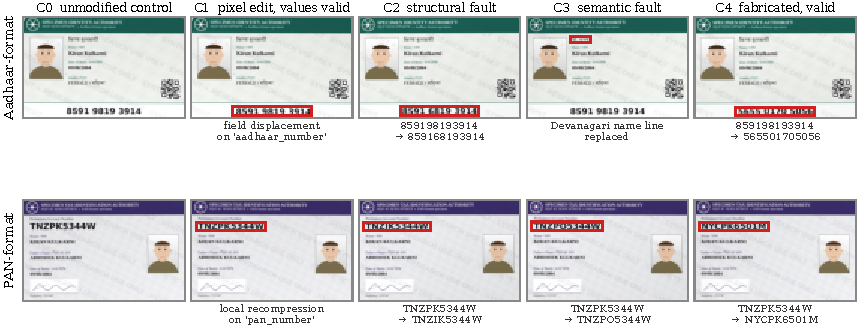
\includegraphics[width=\textwidth]{figures/fig_specimens.pdf}
  \caption{One synthetic identity record rendered across the five forgery
  categories, Aadhaar-format above and PAN-format below, at the clean quality
  tier. The corrupted region is boxed. C1 modifies pixels while leaving every
  printed value valid; C2, C3 and C4 modify a field value and are re-rendered,
  so they carry no pixel-level trace. All identifiers, names and photographs are
  synthetic; the emblem is a placeholder and the authority name is fictitious.}
  \label{fig:specimens}
\end{figure*}

\begin{figure*}[t]
  \centering
  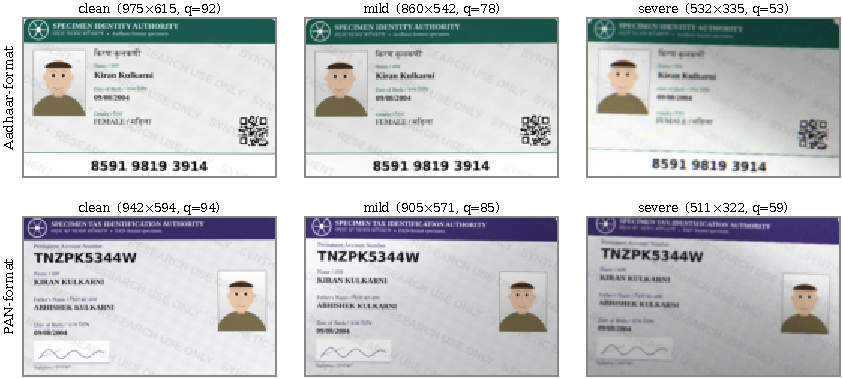
\includegraphics[width=\textwidth]{figures/fig_quality_tiers.pdf}
  \caption{The three capture quality tiers applied to one document, with output
  resolution and JPEG quality factor. Degradation is applied after forgery
  injection and drawn from an identical distribution for every forgery category.}
  \label{fig:qualitytiers}
\end{figure*}

\begin{figure*}[t]
  \centering
  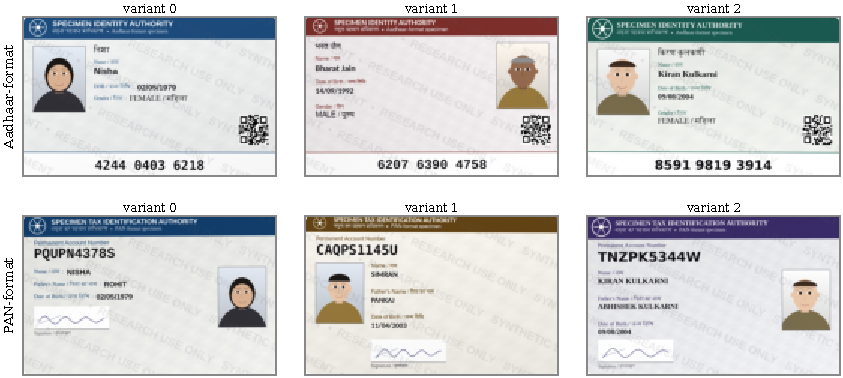
\includegraphics[width=\textwidth]{figures/fig_templates.pdf}
  \caption{The three layout variants per document type. Variants differ in
  typeface pairing, accent colour, label placement, photograph side and
  background pattern density; every variant is present in every split.}
  \label{fig:templates}
\end{figure*}

\subsection{Forgery Taxonomy}
\label{subsec:taxonomy}

Each base record is rendered into six documents: two unmodified controls and one
instance of each of the four forgery categories summarised in
Table~\ref{tab:forgery}.

\textbf{C1} is the only category in which pixels are modified after rendering.
It applies the standard document-tampering repertoire established by
DocTamper~\cite{doctamper} and CMID~\cite{cmid} -- copy-move patch splicing, small
field displacement, font substitution, localised recompression, and patch
resampling -- while leaving every printed value unchanged. The rule branch is
therefore expected to pass on C1, and only the visual branch has anything to
detect. The operation applied and the region affected are recorded per image,
giving localisation ground truth as a by-product.

\textbf{C2}, \textbf{C3} and \textbf{C4} are produced by modifying the identity
record and re-rendering the document through the same pipeline that produces the
controls. The resulting images share the fonts, antialiasing, guilloche phase
and compression history of a genuine render, so the only evidence distinguishing
them from a control is the content of the fields. Producing these categories by
pixel editing would introduce a visual artefact, allow the visual branch to
detect them through that artefact, and invalidate the incremental-value
measurement RQ2 and RQ3 are designed to make. This construction is therefore a
prerequisite of the experimental claim rather than an implementation
convenience.

\textbf{C4 is a deliberate negative control.} Both branches are expected to miss
it: the identifier is fabricated but carries a correctly generated check digit
and a consistent fifth character, so no implemented rule can object to it, and
the document is a genuine render, so no pixel-level trace exists. Reporting the
rate at which the branches do in fact fail on C4 converts the limitation stated
in Section~\ref{sec:framework}-D -- that a passed checksum does not prove
authenticity -- from an assertion into a measurement. One caveat must be carried
into the analysis: because the rule branch also fails on genuine documents
through OCR error (Section~\ref{subsec:characterisation}), a failure on C4 is an
OCR-induced false alarm and \emph{not} detection of the fabrication. Recall on
C4 is therefore not interpretable in isolation, and is reported alongside the
ground-truth-text verdict for the same image so the two causes can be separated.

\textbf{Aadhaar C3 is a deliberate asymmetry control.} Table~\ref{tab:capability} records that Aadhaar supports no cross-field
semantic rule. Omitting C3 from the Aadhaar arm would leave the two document
types with different category sets and would confound RQ5 with a difference in
dataset design. Instead the same \emph{class} of corruption is injected -- the
Latin and Devanagari renderings of the name, which on a genuine document name
the same person, are made to disagree -- and the Aadhaar validator is expected
to miss it, because no implemented rule reads the Devanagari line. RQ5 then
compares like with like: PAN detects this class of inconsistency and Aadhaar
does not, and the difference is attributable to validation capability rather
than to what was put in the dataset.

Before rendering at scale, every validator is run against the ground-truth text
of every generated document, requiring that C0 and C1 pass without exception,
that C2 fail without exception, that C3 fail without exception for PAN and pass
without exception for Aadhaar, and that C4 pass without exception. All
$\dsDocuments$ documents satisfy these conditions; the build aborts otherwise.
A deviation would indicate a generator defect and is not reported as an
experimental result. The complementary check -- that these categories are
visually indistinguishable from a control -- is the subject of
Section~\ref{subsec:probe}.


\subsection{Renderer-Leakage Probe}
\label{sec:dataset-probe}
\label{subsec:probe}

Everything RQ2 and RQ3 measure rests on one assumption: that C2, C3 and C4
documents carry \emph{no} visual evidence of forgery, because they are
re-rendered from a modified record and differ from a genuine control only in
the characters printed in one field. If the rendering pipeline leaked the label
-- through a different code path, a different rasterisation history, or a
layout that reflowed when a field value changed -- a visual detector could
separate those categories from C0 on a rendering artefact, the structural
branch's contribution would appear redundant, and the incremental-value
measurement would be measuring the artefact. The assumption is therefore tested
in two ways rather than asserted, and both tests are reported whatever their
outcome.

\paragraph*{Exact difference audit} C0$_0$, C1, C2, C3 and C4 are rendered from
a single shared render seed, so the guilloche phase, photograph, signature and
placeholder block are identical across them. Before degradation, a forged
document must therefore differ from its genuine control \emph{only} inside the
corrupted field's bounding box, or inside the edited region for C1. This is
checkable exactly rather than statistically: the audit re-renders every
category for \dsProbeRecords{} records, computes the pixel-wise difference
against the control, and counts the pixels that differ outside the expected
region. Over \dsProbeComparisons{} comparisons spanning \dsProbeCells{}
(document type $\times$ category) cells, that count is \textbf{\dsProbeOutside}.
The second control C0$_1$ is drawn with an independent seed, so the corpus is
not reduced to a single background per person.

This audit is not ceremonial. During development it detected a real defect: the
Aadhaar layout advanced each field by the measured extent of the text above it,
so a Devanagari name line of a different height shifted every field below it,
and the C3 script-mismatch category became visually separable through the
resulting reflow rather than through its intended semantic inconsistency. The
renderer was changed to use fixed vertical advances and the corpus regenerated.
A study that had asserted the assumption instead of testing it would have
reported the reflow as a visual-detection result.

\paragraph*{Learned probe} The exact audit governs the renders. The released
images are independently degraded and therefore do differ everywhere, so an
empirical check on them was also run: a gradient-boosted classifier over
downscaled pixels and low-frequency DCT coefficients, trained on the training
split to separate C0 from C2 $\cup$ C3 $\cup$ C4 and evaluated once on the test
split. Its balanced accuracy is \dsProbeCritical{} (95\% CI
\dsProbeCriticalCI, $n=\dsProbeCriticalN$).

That result is reported for completeness and should not be read as
confirmation. A probe too weak to learn anything returns $0.5$ as well, so the
same probe was run as a positive control on C0 versus C1, where a visual cue
exists by construction. It reaches only \dsProbeControl{}
(\dsProbeControlCI, $n=\dsProbeControlN$) over all tiers and
\dsProbeControlClean{} (\dsProbeControlCleanCI,
$n=\dsProbeControlCleanN$) on clean captures alone -- indistinguishable from
chance on a task that is known to be separable. The correct conclusion is that
this probe lacks the statistical power to certify anything, not that the
construction is confirmed: a downscaled-pixel model cannot resolve a font
substitution or a seven-pixel field displacement on a card reduced to fewer
than a hundred pixels on a side.

What carries the claim is therefore the exact difference audit, which is a
proof rather than a statistical test, together with the observation that the
degradation parameters are drawn from a distribution that depends only on the
quality tier and never on the forgery category. A properly powered version of
the probe -- the ResNet-50 branch of Section~\ref{sec:method}-B rather than a
gradient-boosted model over thumbnails -- is reported in
Section~\ref{sec:results}. The construction predicts near-chance performance
there as well, and unlike the probe reported here that prediction will be
falsifiable.

\subsection{Image Quality and Degradation}
\label{subsec:degrade}

Clean renders yield near-perfect OCR and would collapse RQ4 into a degenerate
comparison. Each document is therefore captured at three quality tiers --
\emph{clean}, \emph{mild}, \emph{severe} -- through a seeded capture simulation
implemented directly on NumPy and OpenCV: a single composed homography
(perspective, rotation, scale), an illumination gradient, an optional cast
shadow, optical and occasional motion blur, a moir\'e interference term, sensor
noise, chromatic shift, and JPEG compression at a tier-dependent quality factor.
The released file is the compressed byte stream produced by that last stage, not
a re-encoding of it, so no artificial second compression is layered on top of the
simulated capture. General-purpose document-degradation libraries such as
Augraphy~\cite{augraphy} implement a comparable chain; the pipeline is written here
instead so that the corpus reproduces from the repository with no dependency
beyond NumPy, OpenCV and Pillow, and so that every applied parameter is recorded
per image in the manifest.

Degradation is applied \emph{after} forgery injection, so a C1 pixel edit is
subject to the same degradation as the surrounding document and cannot be
identified by the absence of capture artefacts. The tier is drawn from an
identical distribution for every forgery category, so image quality cannot act
as a class cue. The per-image seed, output resolution and quality factor are
recorded in the manifest.

\subsection{OCR Extraction}
\label{subsec:ocr}

Field values are extracted by cropping to the ground-truth bounding boxes mapped
through the degradation homography and applying Tesseract~\cite{tesseract} per field
with a character whitelist appropriate to the field type. Raw output is stored
without correction. A minimal and explicitly documented \emph{parsing} step is
applied before the validators see a string -- whitespace removal for the two
identifier fields, which are printed in groups, and whitespace normalisation for
name fields -- and nothing else. No character substitution, dictionary lookup,
checksum-guided repair or confidence-based rejection is applied, because the gap
between validator behaviour on ground-truth text and on extracted text
\emph{is} the RQ4 measurement, and repairing the output would destroy it.

The whitelists are flat over the field's character class rather than
position-aware. A position-aware whitelist for PAN -- letters at positions 1--5
and 10, digits at 6--9 -- would eliminate most of the confusions reported in
Section~\ref{subsec:characterisation} and would drive the format check's
false-positive rate towards zero. It would do so by constraining the extractor
with exactly the format the validator then checks, making the format check
partly self-fulfilling and inflating the apparent quality of the structural
branch. The flat whitelist is the conservative choice and is the one used.

Two limitations follow from the available OCR model. Only the English Tesseract
model is used, so the Devanagari name line is rendered but not extracted; the
Aadhaar C3 corruption is consequently unreadable by the pipeline by
construction, which is the intended negative control but also means the Aadhaar
semantic gap is demonstrated rather than closed. Second, a robustness check
against an independent second engine is not performed here; the extraction
interface accepts an alternative engine and this is left to
Section~\ref{sec:discussion-threats} as a stated threat rather than claimed as done.

\subsection{Corpus Characterisation and Validator Behaviour}
\label{subsec:characterisation}

The measurements in this subsection characterise the \emph{corpus} and the rule
branch operating on it. No visual model is trained and no fusion is performed at
this stage, so none of these numbers is a detection result for the hybrid
system; they are the inputs on which Sections~\ref{sec:setup}
and~\ref{sec:results} build, and they establish that the corpus has the
properties the experimental design assumes.

Table~\ref{tab:ocr} and Figure~\ref{fig:ocr} report per-field extraction
quality. The Aadhaar number is recovered exactly on
$\dsOcrAadhaarAadhaarNumberClean\%$ of clean captures and
$\dsOcrAadhaarAadhaarNumberSevere\%$ of severe ones. The PAN number is recovered
on only $\dsOcrPanPanNumberClean\%$ of clean captures, falling to
$\dsOcrPanPanNumberSevere\%$ under severe degradation. The gap between the two
identifier fields at the same capture quality is instructive and is not a
degradation effect: a PAN mixes letters and digits without positional
constraint at the extractor, and the dominant residual errors are the
character-shape confusions $0\!\leftrightarrow\!\mathrm{O}$,
$\mathrm{I}\!\leftrightarrow\!1$ and $5\!\rightarrow\!\mathrm{S}$, together with
occasional insertions that change the string length. An Aadhaar number, being
purely numeric, admits no such confusion.

Table~\ref{tab:rulerate} reports the rule-branch flag rate by category on
ground-truth text and on extracted text. On ground-truth text the branch behaves
exactly as designed: it flags $100\%$ of C2 for both document types and $100\%$
of PAN C3, and $0\%$ of everything else. On extracted text this structure
survives -- C2 and PAN C3 remain near-saturated -- but a floor of spurious
failures appears in every other cell, and that floor is the cost of operating on
real OCR output.

Table~\ref{tab:fpr} isolates that cost on genuine documents, which is the
measurement RQ6 requires. On ground-truth text the false-positive rate is zero
by construction, so every entry is attributable to extraction error. For Aadhaar
it rises from $\dsFPAadhaarClean\%$ on clean captures to
$\dsFPAadhaarSevere\%$ on severe ones. For PAN it is $\dsFPPanClean\%$ even on
clean captures and $\dsFPPanSevere\%$ on severe ones -- an order of magnitude
above Aadhaar at the same capture quality. The asymmetry that
Section~\ref{sec:asymmetry} treats as an advantage for PAN, namely that PAN
supports more independent checks than Aadhaar, is therefore also a liability:
more rules applied to a harder-to-extract field produce more opportunities to
fail on a genuine document. Any fusion rule that treats a structural failure as
evidence of forgery inherits this rate, which is why RQ6 is included in the
question set and why a detection-only evaluation of the hybrid system would not
be interpretable.

Table~\ref{tab:permstrict} separates the permissive rule of~(2) from its strict
variant on genuine PAN documents. On ground-truth text the permissive rule never
fails, as it must not. The strict variant fails on $\dsStrictAll\%$ of all genuine
documents, and that failure is not spread evenly: it is confined entirely to the
initial-first stratum, where it reaches $\dsStrictInitialFirst\%$, and within
that stratum to records whose fifth character derives from the abbreviated
leading token, where it reaches $\dsStrictLeadingInitial\%$. The corpus-level figure depends on the modelling assumption
of Section~\ref{subsec:records} and should be read as conditional on it; the
stratified figures do not. This is the quantity Section~\ref{sec:framework}-B
identified as reportable, and it is the empirical justification for adopting the
permissive rule as this study's primary check: a rule that simply took the last
whitespace-delimited token as the surname would report a semantic failure for
close to one genuine document in three within a naming convention held by a
large population, contaminating exactly the measurement this study is designed
to make.

\begin{table}[t]
\caption{Per-field OCR extraction quality by capture quality tier:
exact-match rate with a 95\% Wilson interval, and mean character
error rate. Raw Tesseract output, with only the parsing step of
Section~\ref{subsec:ocr} applied.}
\label{tab:ocr}
\centering
\footnotesize
\begin{tabular}{@{}llrrr@{}}
\toprule
Field & Tier & $n$ & Exact match \% [95\% CI] & CER \% \\
\midrule
A: number & clean & 1800 & 99.8 [99.5, 99.9] & 0.01 \\
 & mild & 1800 & 99.4 [99.0, 99.7] & 0.07 \\
 & severe & 1800 & 88.3 [86.8, 89.7] & 2.50 \\
\addlinespace[1.5pt]
A: name & clean & 1800 & 98.8 [98.2, 99.2] & 0.10 \\
 & mild & 1800 & 98.7 [98.1, 99.2] & 0.10 \\
 & severe & 1800 & 64.7 [62.5, 66.9] & 22.22 \\
\addlinespace[1.5pt]
A: DOB & clean & 1800 & 100.0 [99.8, 100.0] & 0.00 \\
 & mild & 1800 & 100.0 [99.8, 100.0] & 0.00 \\
 & severe & 1800 & 41.5 [39.2, 43.8] & 45.33 \\
\addlinespace[1.5pt]
P: number & clean & 1800 & 85.2 [83.5, 86.7] & 1.57 \\
 & mild & 1800 & 84.9 [83.2, 86.5] & 1.57 \\
 & severe & 1800 & 67.7 [65.5, 69.8] & 7.30 \\
\addlinespace[1.5pt]
P: name & clean & 1800 & 99.7 [99.3, 99.8] & 0.04 \\
 & mild & 1800 & 99.6 [99.2, 99.8] & 0.06 \\
 & severe & 1800 & 53.8 [51.5, 56.1] & 31.78 \\
\addlinespace[1.5pt]
P: father & clean & 1800 & 100.0 [99.8, 100.0] & 0.00 \\
 & mild & 1800 & 100.0 [99.8, 100.0] & 0.00 \\
 & severe & 1800 & 44.7 [42.4, 47.0] & 43.68 \\
\addlinespace[1.5pt]
P: DOB & clean & 1800 & 99.7 [99.3, 99.9] & 0.03 \\
 & mild & 1800 & 99.9 [99.7, 100.0] & 0.01 \\
 & severe & 1800 & 33.8 [31.7, 36.0] & 50.84 \\
\bottomrule
\end{tabular}
\end{table}

\begin{table}[t]
\caption{Rule-branch flag rate by forgery category (\% of images on
which an applicable rule evaluated \textsc{false}), on ground-truth
text and on OCR-extracted text, with 95\% Wilson intervals. On C0 a
flag is a false positive. On C4 both branches are expected to miss by
construction, so a flag there is an OCR-induced false alarm and not
detection of the fabrication.}
\label{tab:rulerate}
\centering
\footnotesize
\begin{tabular}{@{}llll@{}}
\toprule
Document & Cat. & Ground-truth text & OCR text \\
\midrule
Aadhaar & C0 & 0.0 [0.0, 0.2] & 4.1 [3.3, 5.1] \\
 & C1 & 0.0 [0.0, 0.4] & 4.1 [3.0, 5.6] \\
 & C2 & 100.0 [99.6, 100.0] & 99.8 [99.2, 99.9] \\
 & C3 & 0.0 [0.0, 0.4] & 3.9 [2.8, 5.4] \\
 & C4 & 0.0 [0.0, 0.4] & 4.0 [2.9, 5.5] \\
\midrule
PAN & C0 & 0.0 [0.0, 0.2] & 18.9 [17.1, 20.8] \\
 & C1 & 0.0 [0.0, 0.4] & 20.8 [18.3, 23.5] \\
 & C2 & 100.0 [99.6, 100.0] & 97.1 [95.8, 98.0] \\
 & C3 & 100.0 [99.6, 100.0] & 96.2 [94.8, 97.3] \\
 & C4 & 0.0 [0.0, 0.4] & 23.2 [20.6, 26.1] \\
\bottomrule
\end{tabular}
\end{table}

\begin{table}[t]
\caption{Rule-branch false-positive rate on \emph{genuine} documents
(category C0) as a function of capture quality, evaluated on
OCR-extracted text. On ground-truth text the rate is zero by
construction, so every entry here is attributable to OCR extraction
error. This is the measurement RQ6 requires.}
\label{tab:fpr}
\centering
\footnotesize
\begin{tabular}{@{}llrrl@{}}
\toprule
Document & Tier & $n$ & FP & FP rate \% [95\% CI] \\
\midrule
Aadhaar & clean & 600 & 2 & 0.3 [0.1, 1.2] \\
 & mild & 600 & 2 & 0.3 [0.1, 1.2] \\
 & severe & 600 & 70 & 11.7 [9.3, 14.5] \\
 & all & 1800 & 74 & 4.1 [3.3, 5.1] \\
\midrule
PAN & clean & 600 & 76 & 12.7 [10.2, 15.6] \\
 & mild & 600 & 73 & 12.2 [9.8, 15.0] \\
 & severe & 600 & 191 & 31.8 [28.2, 35.7] \\
 & all & 1800 & 340 & 18.9 [17.1, 20.8] \\
\bottomrule
\end{tabular}
\end{table}

\begin{table}[t]
\caption{PAN cross-field rule on \emph{genuine} documents:
permissive rule (2) against the strict variant, by naming stratum and
by the source of the fifth character. A failure here is a false
positive on a genuine document. The strict variant is reported as a
sensitivity analysis, not as the study's rule.}
\label{tab:permstrict}
\centering
\scriptsize
\setlength{\tabcolsep}{3.5pt}
\begin{tabular}{@{}llrll@{}}
\toprule
Subset & Text & $n$ & Permissive FAIL \% & Strict FAIL \% \\
\midrule
all genuine PAN & gt & 1800 & 0.0 [0.0, 0.2] & 9.0 [7.8, 10.4] \\
 & ocr & 1800 & 1.9 [1.4, 2.6] & 9.4 [8.2, 10.9] \\
\addlinespace[1.5pt]
surname-last & gt & 648 & 0.0 [0.0, 0.6] & 0.0 [0.0, 0.6] \\
 & ocr & 648 & 1.1 [0.5, 2.2] & 1.4 [0.7, 2.6] \\
\addlinespace[1.5pt]
initial-first & gt & 552 & 0.0 [0.0, 0.7] & 29.3 [25.7, 33.3] \\
 & ocr & 552 & 3.8 [2.5, 5.7] & 27.4 [23.8, 31.2] \\
\addlinespace[1.5pt]
mononymic & gt & 600 & 0.0 [0.0, 0.6] & 0.0 [0.0, 0.6] \\
 & ocr & 600 & 1.0 [0.5, 2.2] & 1.7 [0.9, 3.0] \\
\addlinespace[1.5pt]
$p_5$ from initial & gt & 174 & 0.0 [0.0, 2.2] & 93.1 [88.3, 96.0] \\
 & ocr & 174 & 6.9 [4.0, 11.7] & 81.0 [74.6, 86.2] \\
\addlinespace[1.5pt]
$p_5$ from given name & gt & 378 & 0.0 [0.0, 1.0] & 0.0 [0.0, 1.0] \\
 & ocr & 378 & 2.4 [1.3, 4.5] & 2.6 [1.4, 4.8] \\
\addlinespace[1.5pt]
\bottomrule
\end{tabular}
\end{table}


\begin{figure}[t]
  \centering
  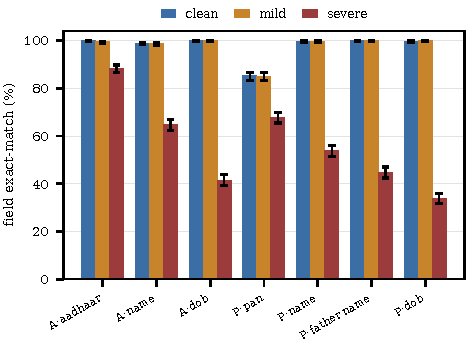
\includegraphics[width=\columnwidth]{figures/fig_ocr_quality.pdf}
  \caption{Per-field OCR exact-match rate by capture quality tier, with $95\%$
  Wilson intervals. ``A'' denotes Aadhaar-format fields and ``P'' PAN-format
  fields.}
  \label{fig:ocr}
\end{figure}

\subsection{Train/Validation/Test Split and Leakage Control}
\label{subsec:leakage}

Splits are made at the level of the person identifier, not the image and not the
document, and stratified over the naming stratum and both template-variant
assignments. An image-level split would place one identity's genuine and forged
documents on opposite sides of the partition, allowing a model to recognise the
identity rather than the forgery. Allocation uses a running largest-deficit rule
rather than per-stratum integer flooring, which at this number of strata would
systematically starve the two minority splits; the realised partition is
$\dsTrainPer/\dsValPer/\dsTestPer$ persons and
$\dsTrainImg/\dsValImg/\dsTestImg$ images. Fusion thresholds
(Section~\ref{sec:method}-E) are calibrated on the validation split only; the
test split is evaluated once.

Five leakage modes are audited on the released splits and the audit is reported
in Table~\ref{tab:leakage} rather than asserted. Four are exact and all pass: no
person identifier, no Aadhaar or PAN string, and no set of printed field values
occurs in more than one split, and no document's degradation draws span splits.

The fifth, near-duplicate detection by perceptual hashing, is reported as a
\emph{diagnostic rather than a gate}, because running it establishes that it
cannot serve as one here. Every document in this corpus shares one of six card
layouts, which dominates the low-frequency DCT band a perceptual hash is built
from. A $64$-bit hash is degenerate on this corpus: it yields only
$\dsPhashDistinctSixtyFour$ distinct values for $\dsImages$ images and collides
across different persons, different forgery categories and different splits. A
$\dsPhashBits$-bit hash separates images ($\dsPhashDistinct$ distinct values) but
still does not cleanly separate identities: the median distance between two
captures of the same document is $\dsPhashWithinMed$ bits and between two
different persons' documents $\dsPhashCrossPersonMed$ bits, but the
distributions overlap, with separability AUC $\dsPhashAUC$ and
$\dsPhashOverlap\%$ of different-person pairs closer than the median
same-document pair. No distance threshold can therefore distinguish a leaked
duplicate from two unrelated documents on the same template, and the smallest
cross-split distances are additionally a minimum taken over every training
image, which is small for that reason alone. Because the exact identity audit
already establishes that the splits are person-disjoint, every cross-split
neighbour is necessarily a different person, and these distances carry no
leakage information beyond what that audit establishes.
Figure~\ref{fig:phash} shows the three distance distributions. Reporting this
negatively is preferable to reporting a threshold-based pass that the measure
does not support.

\begin{table}[t]
\caption{Leakage audit performed on the released splits. Each check is
run on the corpus and its outcome reported, rather than asserted. The
first four checks are exact and all pass. The fifth, near-duplicate
detection by perceptual hashing, is reported as a \emph{diagnostic}
rather than a gate: on a corpus in which every document shares one
of six layout templates, the same-document and different-person
distance distributions overlap, so no threshold can separate a
leaked duplicate from two unrelated documents. See
Section~\ref{subsec:leakage} and Fig.~\ref{fig:phash}.}
\label{tab:leakage}
\centering
\scriptsize
\setlength{\tabcolsep}{3.5pt}
\begin{tabular}{@{}p{1.15cm}p{3.0cm}ll@{}}
\toprule
Leakage mode & Check & Required & Observed \\
\midrule
Identity & person-id intersection across splits & empty & 0 \\
Identifier & Aadhaar/PAN string intersection & empty & 0 \\
Template & every layout variant in every split & all & 6/6 \\
Near-duplicate & \dsPhashBits-bit perceptual-hash distance & (diagnostic) & see Sec.~\ref{subsec:leakage} \\
Augment\-ation & degradation draws of one document & one split & 0 span splits \\
Printed values & identical field-value set in two splits & none & 0 of 2100 \\
\bottomrule
\end{tabular}
\end{table}


\begin{figure}[t]
  \centering
  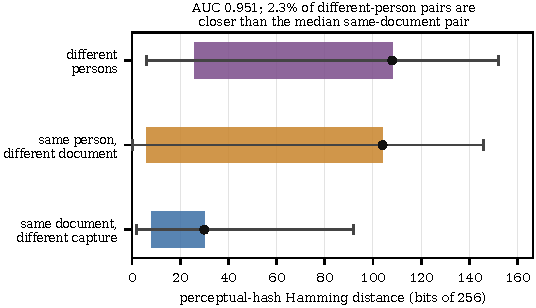
\includegraphics[width=\columnwidth]{figures/fig_phash_leakage.pdf}
  \caption{Perceptual-hash distance distributions ($\dsPhashBits$-bit hash);
  bars span the first percentile to the median, whiskers the full range, dots
  the median. The same-document and different-person distributions overlap, so
  the near-duplicate check is reported as a diagnostic and the leakage verdict
  rests on the exact audits of Table~\ref{tab:leakage}.}
  \label{fig:phash}
\end{figure}


\subsection{Reproducibility and Release}
\label{subsec:release}

The dataset is reproducible from code. A single entry point regenerates
templates, identifiers, renders, forgeries, degradations, OCR output, splits,
audits and figures from one global seed, with dependency versions pinned, the
font binaries committed to the repository so that rasterisation does not depend
on the host system's installed faces, and the OCR binary version recorded. The
number of worker processes does not affect the output, because every random draw
is seeded from the person identifier rather than from execution order. Build
time is approximately $17$ minutes on two cores and the corpus occupies
$\dsGiB$\,GiB.

The release comprises the generation code, the configuration, the manifest and
the figures, from which the image corpus can be regenerated exactly; the built
corpus is additionally archived. The manifest records, per image: the image,
document and person identifiers; document type, forgery category, quality tier,
naming stratum, template variant and split; ground-truth and extracted field
values with per-field exact-match and character error rate; field bounding boxes
in the degraded image's coordinate frame; the corrupted field with its values
before and after; the C1 operation and its region; the render and degradation
seeds; and the validator output on both ground-truth and extracted text.

\subsection{Ethical Considerations}
\label{subsec:ethics}

No real Aadhaar or PAN document, image or number was collected, downloaded,
purchased or processed at any stage. All identifiers are synthetic. No
identifier was submitted to or verified against any government or third-party
identity service. No official emblem is reproduced; a visually distinct
placeholder mark is used in its place, the issuing authority named on the cards
is fictitious, and every image carries a permanent synthetic-specimen overlay.

As Section~\ref{subsec:identifiers} establishes quantitatively, a small
proportion of the generated identifiers can be expected to coincide with issued
ones, and it would be false to claim otherwise. The case that the release is
nonetheless safe rests on non-linkage rather than on non-coincidence. A bare
identifier string carrying no association to a real person is not information
about an identifiable person; in this corpus every identifier is printed
alongside a generated name, a generated date of birth and a procedurally drawn
placeholder, none of which belongs to any human being, so a coincident number
appears in the dataset attached to a person who does not exist. No identifier was
ever resolved or verified, so the corpus contains no information about whether
any string is issued and none about any holder. The expected coincidence count
is reported rather than suppressed, so a user of the dataset can reason about it
directly.

The released artefacts are intended to support evaluation of forgery
\emph{detection} and are not sufficient to produce a document capable of passing
any operational verification process, since structural validity is explicitly
shown in this study -- by category C4 -- not to establish authenticity.
